\documentclass[a4paper]{article}

% Compile from this directory (LM/report/):
%   latexmk -pdf report_LM.tex
% The style files are picked up from ../../report_template/.
\usepackage{../../report_template/INTERSPEECH2021}
\usepackage{booktabs}
\usepackage{pgfplots}
\pgfplotsset{compat=1.14}

% Colorblind-safe palette (Okabe-Ito): blue for validation, vermillion for test, green for LoRA.
\definecolor{cbblue}{HTML}{0072B2}
\definecolor{cbverm}{HTML}{D55E00}
\definecolor{cbgreen}{HTML}{009E73}

% Self-contained bibliography: this block writes lm_refs.bib at compile time.
\begin{filecontents*}[overwrite]{lm_refs.bib}
@article{radford2019gpt2,
  author  = {Alec Radford and Jeffrey Wu and Rewon Child and David Luan and Dario Amodei and Ilya Sutskever},
  title   = {Language Models are Unsupervised Multitask Learners},
  journal = {OpenAI Technical Report},
  year    = {2019}
}
@inproceedings{vaswani2017attention,
  author    = {Ashish Vaswani and Noam Shazeer and Niki Parmar and Jakob Uszkoreit and Llion Jones and Aidan N. Gomez and Lukasz Kaiser and Illia Polosukhin},
  title     = {Attention Is All You Need},
  booktitle = {Advances in Neural Information Processing Systems},
  year      = {2017}
}
@article{marcus1993ptb,
  author  = {Mitchell P. Marcus and Beatrice Santorini and Mary Ann Marcinkiewicz},
  title   = {Building a Large Annotated Corpus of {English}: The {Penn Treebank}},
  journal = {Computational Linguistics},
  volume  = {19},
  number  = {2},
  pages   = {313--330},
  year    = {1993}
}
@inproceedings{hu2022lora,
  author    = {Edward J. Hu and Yelong Shen and Phillip Wallis and Zeyuan Allen-Zhu and Yuanzhi Li and Shean Wang and Lu Wang and Weizhu Chen},
  title     = {{LoRA}: Low-Rank Adaptation of Large Language Models},
  booktitle = {International Conference on Learning Representations},
  year      = {2022}
}
@article{srivastava2014dropout,
  author  = {Nitish Srivastava and Geoffrey Hinton and Alex Krizhevsky and Ilya Sutskever and Ruslan Salakhutdinov},
  title   = {Dropout: A Simple Way to Prevent Neural Networks from Overfitting},
  journal = {Journal of Machine Learning Research},
  volume  = {15},
  pages   = {1929--1958},
  year    = {2014}
}
@inproceedings{press2017tying,
  author    = {Ofir Press and Lior Wolf},
  title     = {Using the Output Embedding to Improve Language Models},
  booktitle = {Proceedings of EACL},
  year      = {2017}
}
\end{filecontents*}

% Lab 4: Language Modeling (parts 1.A and 1.B)
\title{NLU course project: Language Modeling (Lab 4)}
\name{Kevin Shimaj (mat. 267432)}

\address{
  University of Trento}
\email{kevin.shimaj@studenti.unitn.it}

\begin{document}

\maketitle

\section{Introduction}
This report covers the two language modeling tasks on the Penn Treebank (PTB) corpus \cite{marcus1993ptb}. In part 1.A a GPT-2 style decoder \cite{radford2019gpt2} is trained from scratch, starting from the tiny lab baseline and growing it one hyperparameter at a time; a change is kept only when the validation perplexity (PPL) improves, and every run is reported, including the rejected ones. The final model (256 hidden size, 8 heads, 6 layers, dropout 0.2) reaches a test PPL of 30.39, well below the 250 target; weight tying was also implemented and evaluated, but rejected after four controlled runs. In part 1.B the pretrained GPT-2 is adapted to PTB by training only hand-written LoRA adapters \cite{hu2022lora} on the attention projections, with the constraint of beating the part 1.A result. The adapted model reaches a test PPL of 20.61, below both the target and the part 1.A score, while updating only 0.35\% of the weights.

\section{Implementation details}
\textbf{Part 1.A.} All runs share the lab protocol: GPT-2 BPE tokenizer (pad token set to eos), next-token prediction with inputs and labels shifted by one, token-weighted cross entropy, AdamW, batch size 8 for training and 16 for evaluation, early stopping with patience 3 on validation PPL. PPL is the exponential of the token-weighted mean loss, and the reported test score is always the one of the best validation checkpoint. The search had three phases. (i) A learning rate sweep on the tiny baseline over $\{5\mathrm{e}{-4}, 1\mathrm{e}{-3}, 2\mathrm{e}{-3}, 5\mathrm{e}{-3}\}$, a log-spaced grid centered on the stable AdamW range; the lab value $0.1$ is unstable and stalls at high PPL. (ii) Architecture growth, one knob at a time: $d_{\mathrm{model}}$ from 20 to 256 (384 hurt; the embedding table dominates the parameter count, so width saturates first), heads from 1 to 8 (almost free, since they only reshape the attention projections), layers from 1 to 6 (gains shrink geometrically), and feed-forward size from 20 to 1024, i.e. $4 \times d_{\mathrm{model}}$ as in the standard Transformer \cite{vaswani2017attention}, which gave the largest single improvement. (iii) A second sweep on the final architecture, where $2\mathrm{e}{-3}$ won: this model overfits PTB in a few epochs, and under early stopping the gradient noise of a higher rate works as an implicit regularizer. The value $5\mathrm{e}{-3}$ was not rerun because it was already the worst point of the first sweep and deeper networks are less tolerant to large steps. (iv) Dropout \cite{srivastava2014dropout} at the four lab locations: after the summed embeddings, on the attention weights after the softmax, after the attention output projection, and in the feed-forward block after the activation and after the last linear layer. It pays here precisely because the final model overfits PTB within a few epochs: $p{=}0.1$ gains 2 validation PPL and $p{=}0.2$ another 1.3, with training surviving more epochs before early stopping (22 vs 10). (v) Weight tying \cite{press2017tying} shares the embedding matrix with the output head ($-12.9$M parameters). It interacts badly with the lab initialization: the uniform re-init of the head silently flattens the tied embeddings to near zero and training stalls. Re-initializing token and positional embeddings at the GPT-2 scale, $\mathcal{N}(0, 0.02)$, restores a healthy start, but convergence then crawls towards a plateau roughly 15 PPL above the untied model --- identically at both dropout levels, so the cost is the shared input/output geometry itself and not an excess of regularization. The tie was therefore reverted.

\textbf{Part 1.B.} The whole pretrained model is frozen and each attention block gets a low-rank adapter on the Q, K, V projections: the output becomes $Wx + B(A(x))\,\alpha/r$, with $A$ initialized from a normal distribution and $B$ at zero, so training starts exactly at the pretrained weights and only the adapters are updated. The search followed the idea behind LoRA, that the weight update needed to adapt a large model has a low intrinsic rank. It started from a small rank of 8 with the scale $\alpha$ set equal to the rank, which is the neutral choice. This first setting already passed both targets, so the effort moved to the learning rate: $1\mathrm{e}{-3}$ improved over $5\mathrm{e}{-4}$, which fits the fact that updating only a small fraction of the weights tolerates a larger step. Higher ranks were not explored, since a low intrinsic rank means that extra capacity is expected to help little while doubling or quadrupling the adapter size.

\section{Results}
Table~\ref{tab:parta} lists every part 1.A run in chronological order. Figure~\ref{fig:ladder} shows the chain of accepted steps: capacity dominates at the start (width, then depth), the feed-forward expansion gives the largest single architectural drop ($-3.4$ validation PPL), consistent with the fact that a 20-unit MLP was a strong bottleneck for 256-dimensional states, and the two dropout steps close the ladder with a further $-3.3$. The four weight-tying runs (19--22 in the table) were all rejected: two stalled because of the initialization interaction described above and two converged healthily but towards a far worse plateau, so they were aborted once the trajectory was clearly dominated (their dev column reports the last value before the manual stop). Figure~\ref{fig:lr} compares the two learning rate sweeps: the optimum moves from $1\mathrm{e}{-3}$ on the tiny model to $2\mathrm{e}{-3}$ on the final one, while the low end ($5\mathrm{e}{-4}$) gets clearly worse, which supports the regularization reading given above. Note that test PPL is consistently below validation PPL on PTB; this is a property of the split, not a bug. Table~\ref{tab:partb} reports part 1.B. Both settings clear the targets by a wide margin, and the final adapter reaches a test PPL of 20.61 against the 30.39 of part 1.A while updating only 0.35\% of the parameters. This large gap is expected: part 1.B starts from a model already pretrained on a much larger corpus and only shifts it towards PTB, whereas part 1.A learns the language from scratch on the small PTB training set.

% Keep the one-page body on page 1; send all tables, figures and references to page 2.
\clearpage

\begin{table}[t]
  \centering
  \caption{Part 1.A, full incremental log. Config is $d_{\mathrm{model}}$/heads/layers/ff. Decision: K = kept, R = rejected (reverted). In runs 20--21 ``init .02'' is the $\mathcal{N}(0, 0.02)$ re-init of the tied token (and positional) embeddings. $^\dagger$: run aborted once clearly dominated; value is the validation PPL at the manual stop (after 8, 1, 25 and 9 epochs respectively).}
  \label{tab:parta}
  \scriptsize
  \begin{tabular}{@{}rllllll@{}}
    \toprule
    \# & Step & Config & lr & Dev & Test & D \\
    \midrule
    1  & baseline (lab)   & 20/1/1/20      & $0.1$              & 95.45 & 82.97 & -- \\
    2  & lr sweep         & 20/1/1/20      & $1\mathrm{e}{-3}$  & 51.93 & 45.28 & K \\
    3  & lr sweep         & 20/1/1/20      & $2\mathrm{e}{-3}$  & 52.32 & 46.07 & R \\
    4  & lr sweep         & 20/1/1/20      & $5\mathrm{e}{-3}$  & 53.62 & 47.08 & R \\
    5  & lr sweep         & 20/1/1/20      & $5\mathrm{e}{-4}$  & 52.40 & 45.44 & R \\
    6  & $d_{\mathrm{model}}$ & 128/1/1/20 & $1\mathrm{e}{-3}$  & 45.68 & 40.70 & K \\
    7  & $d_{\mathrm{model}}$ & 256/1/1/20 & $1\mathrm{e}{-3}$  & 45.53 & 40.74 & K \\
    8  & $d_{\mathrm{model}}$ & 384/1/1/20 & $1\mathrm{e}{-3}$  & 45.73 & 40.65 & R \\
    9  & heads            & 256/4/1/20     & $1\mathrm{e}{-3}$  & 43.55 & 39.13 & K \\
    10 & heads            & 256/8/1/20     & $1\mathrm{e}{-3}$  & 43.47 & 39.11 & K \\
    11 & layers           & 256/8/2/20     & $1\mathrm{e}{-3}$  & 42.25 & 38.05 & K \\
    12 & layers           & 256/8/4/20     & $1\mathrm{e}{-3}$  & 41.34 & 37.21 & K \\
    13 & layers           & 256/8/6/20     & $1\mathrm{e}{-3}$  & 40.82 & 36.90 & K \\
    14 & ff ($4 \times d$) & 256/8/6/1024  & $1\mathrm{e}{-3}$  & 37.39 & 33.92 & K \\
    15 & lr re-tune       & 256/8/6/1024   & $5\mathrm{e}{-4}$  & 39.12 & 35.14 & R \\
    16 & lr re-tune       & 256/8/6/1024   & $2\mathrm{e}{-3}$  & 37.09 & 33.68 & K \\
    17 & dropout $p{=}0.1$ & 256/8/6/1024  & $2\mathrm{e}{-3}$  & 35.07 & 31.65 & K \\
    18 & dropout $p{=}0.2$ & 256/8/6/1024  & $2\mathrm{e}{-3}$  & \textbf{33.79} & \textbf{30.39} & K \\
    19 & tie, lab init     & 256/8/6/1024  & $2\mathrm{e}{-3}$  & 151$^\dagger$ & -- & R \\
    20 & tie, init .02 (tok) & 256/8/6/1024 & $2\mathrm{e}{-3}$ & 241$^\dagger$ & -- & R \\
    21 & tie, init .02 (tok+pos) & 256/8/6/1024 & $2\mathrm{e}{-3}$ & 48.4$^\dagger$ & -- & R \\
    22 & tie + drop $p{=}0.1$ & 256/8/6/1024 & $2\mathrm{e}{-3}$ & 57.5$^\dagger$ & -- & R \\
    \bottomrule
  \end{tabular}
\end{table}

\begin{table}[t]
  \centering
  \caption{Part 1.B, LoRA fine-tuning of pretrained GPT-2 on PTB. Reference to beat: test PPL 30.39 (part 1.A). Trainable is the share of updated weights. Decision: K = kept, R = rejected.}
  \label{tab:partb}
  \footnotesize
  \begin{tabular}{@{}rlllllll@{}}
    \toprule
    \# & rank & $\alpha$ & lr & Trainable & Dev & Test & D \\
    \midrule
    1 & 8 & 8 & $5\mathrm{e}{-4}$ & 0.35\% & 23.36 & 21.11 & R \\
    2 & 8 & 8 & $1\mathrm{e}{-3}$ & 0.35\% & \textbf{22.83} & \textbf{20.61} & K \\
    \bottomrule
  \end{tabular}
\end{table}

\begin{figure}[t]
  \centering
  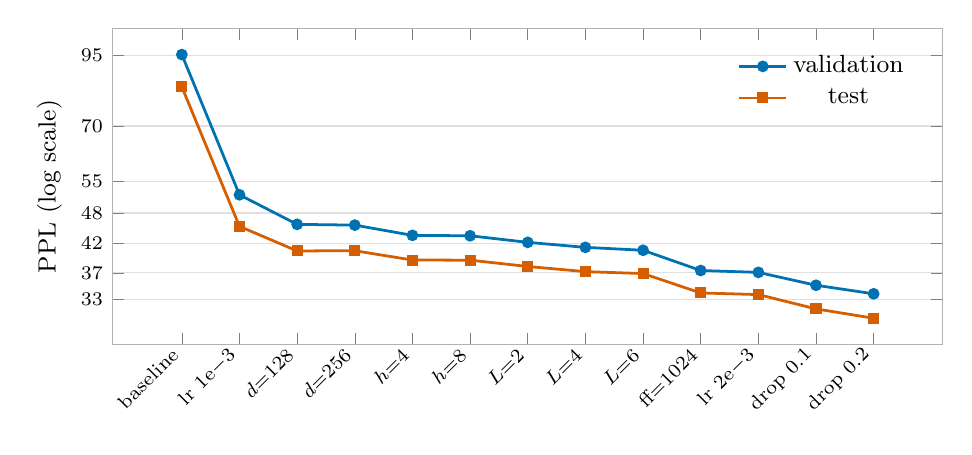
\begin{tikzpicture}
    \begin{axis}[
      width=\columnwidth, height=5.6cm,
      ymode=log, log ticks with fixed point,
      ytick={33,37,42,48,55,70,95},
      xtick={1,2,3,4,5,6,7,8,9,10,11,12,13},
      xticklabels={baseline, lr $1\mathrm{e}{-3}$, $d$=128, $d$=256, $h$=4, $h$=8, $L$=2, $L$=4, $L$=6, ff=1024, lr $2\mathrm{e}{-3}$, drop 0.1, drop 0.2},
      x tick label style={rotate=45, anchor=east, font=\scriptsize},
      ylabel={PPL (log scale)},
      ymajorgrids, grid style={gray!25},
      axis line style={gray!60},
      tick label style={font=\scriptsize},
      label style={font=\small},
      legend style={draw=none, fill=none, font=\small, at={(0.97,0.95)}, anchor=north east},
    ]
      \addplot[color=cbblue, mark=*, mark size=1.6, line width=1pt]
        coordinates {(1,95.45)(2,51.93)(3,45.68)(4,45.53)(5,43.55)(6,43.47)(7,42.25)(8,41.34)(9,40.82)(10,37.39)(11,37.09)(12,35.07)(13,33.79)};
      \addplot[color=cbverm, mark=square*, mark size=1.5, line width=1pt]
        coordinates {(1,82.97)(2,45.28)(3,40.70)(4,40.74)(5,39.13)(6,39.11)(7,38.05)(8,37.21)(9,36.90)(10,33.92)(11,33.68)(12,31.65)(13,30.39)};
      \legend{validation, test}
    \end{axis}
  \end{tikzpicture}
  \vspace{2mm}
  \caption{Part 1.A: perplexity along the chain of accepted steps. Each point is the run that was kept at that stage of the search (rejected runs are in Table~\ref{tab:parta}).}
  \label{fig:ladder}
\end{figure}

\begin{figure}[t]
  \centering
  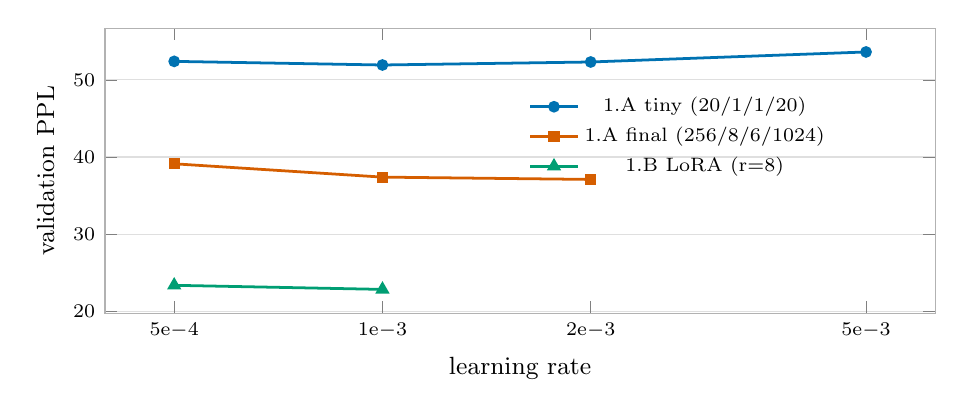
\begin{tikzpicture}
    \begin{axis}[
      width=\columnwidth, height=5.2cm,
      xmode=log,
      xlabel={learning rate}, ylabel={validation PPL},
      xtick={0.0005,0.001,0.002,0.005},
      xticklabels={$5\mathrm{e}{-4}$,$1\mathrm{e}{-3}$,$2\mathrm{e}{-3}$,$5\mathrm{e}{-3}$},
      ymajorgrids, grid style={gray!25},
      axis line style={gray!60},
      tick label style={font=\scriptsize},
      label style={font=\small},
      legend style={draw=none, fill=none, font=\scriptsize, at={(0.5,0.62)}, anchor=west},
    ]
      \addplot[color=cbblue, mark=*, mark size=1.6, line width=1pt]
        coordinates {(0.0005,52.40)(0.001,51.93)(0.002,52.32)(0.005,53.62)};
      \addplot[color=cbverm, mark=square*, mark size=1.5, line width=1pt]
        coordinates {(0.0005,39.12)(0.001,37.39)(0.002,37.09)};
      \addplot[color=cbgreen, mark=triangle*, mark size=2, line width=1pt]
        coordinates {(0.0005,23.36)(0.001,22.83)};
      \legend{1.A tiny (20/1/1/20), 1.A final (256/8/6/1024), 1.B LoRA (r=8)}
    \end{axis}
  \end{tikzpicture}
  \caption{Learning rate sweeps. For part 1.A the optimum moves from $1\mathrm{e}{-3}$ on the tiny model to $2\mathrm{e}{-3}$ on the final one, since the larger model overfits quickly and a higher rate with early stopping generalizes better. Part 1.B, the LoRA fine-tuning, sits much lower and prefers $1\mathrm{e}{-3}$, as adapting only a small fraction of the weights tolerates a larger step.}
  \label{fig:lr}
\end{figure}

\bibliographystyle{../../report_template/IEEEtran}

\bibliography{lm_refs}

\end{document}

